% !TEX root = ../../main.tex

\chapter{Cost Estimation}

\label{chapter:cost-estimation}
In this chapter, we share the results of our experiments and explain they are used for constructing four different cost models. The \hyperref[sec:5-motivation]{first section} shows the results of the runtime experiments, motivating why a cost model is necessary. In the \hyperref[sec:5-gpu-performance-analysis]{next section} the collected profiling metrics are aggregated and analysed, giving insight into how differences between GPUs can affect the trade-off. \autoref{sec:5-feature-engineering} details the process of aggregating and enriching our results to generate an appropriate dataset for the estimators to train on. In \autoref{sec:5-cost-models}, we talk about how we used the enriched results, from the runtime and profiling experiments, to create the cost models. Each model is made for a specific purpose and offers different ways to solve the problem. This chapter aims to give a clear picture of how we ran the experiments and built the cost models from the results.

\section{Motivation}
\label{sec:5-motivation}
This section shows why there is a need for accurate cost estimation for choosing between factorization and materialization. We motivate in three stages. First the benefit of factorization is shown, second we show the impact of data \& model characteristics. By visualizing the performance ratio ($\frac{\text{Time}_M}{\text{Time}_F}$) against a range of independent variables we uncover the first trends that influence the F/M trade-off. Last, we show why GPUs are an important dimension to consider. All figures and values in this section are created with the data collected with the experiments on synthetic datasets, unless specified otherwise.

\subsection{Benefit of factorization}
\begin{figure}[ht]
    \centering
    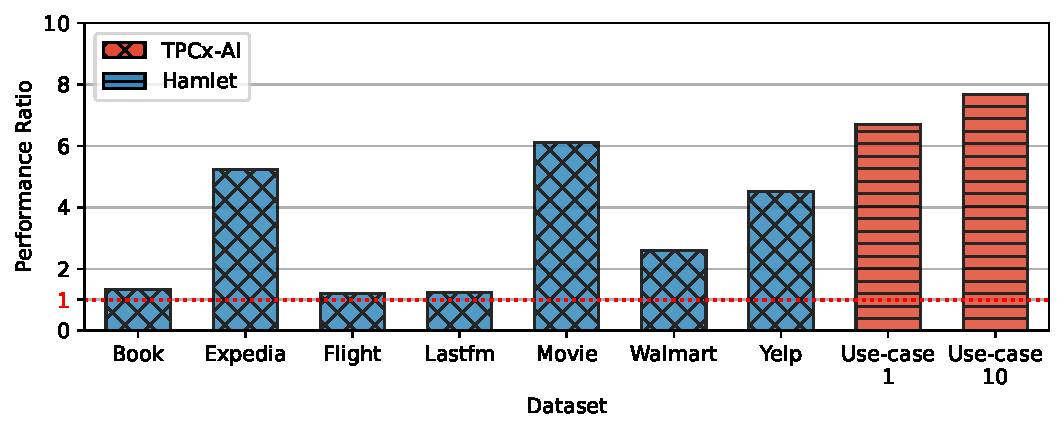
\includegraphics[width=0.7\linewidth]{chapters/05_cost_estimation/figures/real_datasets_speedup.pdf}
    \vspace*{-5mm}
    \caption[Performance gain with factorization on real datasets]{Average Performance ratio of ML models for positive cases ($\text{Time}_M > \text{Time}_F$), split per tested real dataset.}
    \label{fig:5-real-perf-ratio}
\end{figure}

The goal of factorized ML is reducing the number of redundant operations performed during training of a model, to make this process more efficient, i.e., faster. We show the performance gain of factorization over materialization, on real datasets, in \autoref{fig:5-real-perf-ratio}. This shows that exploring factorization is beneficial, as for those cases where it is faster (which is $18\%$ of the tested cases on real datasets), the average speedup is $5.1\times$. In the most extreme cases the training time is reduced by more than $20$ seconds, a reduction by a factor of $27$. In scenarios where training occurs often, e.g., during hyperparameter optimization or online learning this can lead to significant time savings.

% We group the Data and Model characteristics as they both influence the actual computations being executed. The hardware characteristics influence how these computations are carried out on the hardware and are discussed separately. 

\subsection{Data \& Model Characteristics}
\begin{figure}[ht]
    \centering
    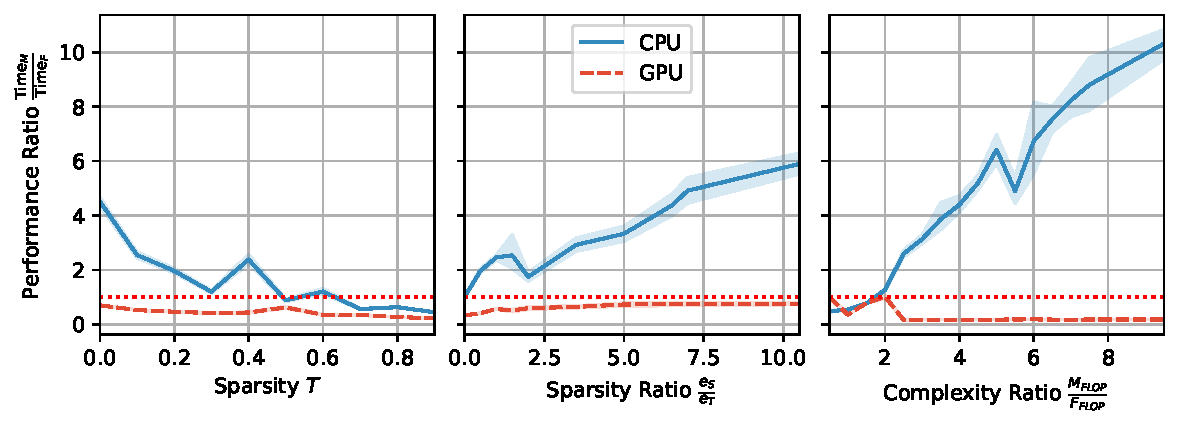
\includegraphics[width=\linewidth]{chapters/05_cost_estimation/figures/motivation_perf_ratio_vs_data_chars.pdf}
    \caption[Performance ratio for various data characteristics]{Performance ratio against various data characteristics. Broken down by compute type (CPU/GPU) and operator type (ML models in the first row \& regular operators in the second). $99\%$ confidence interval shown as shaded area. The sparsity ratio is defined as the sparsity of the source tables $S_k, k\in[1,n]$ divided by the sparsity of target table $T$. Sparsity of $S$ is defined as the total non-zero values in the base tables divided by the total number of cells in the base tables, $\frac{\sum_{k=1}^{n} nnz(S_k)}{\sum_{k=1}^{n} r_{S_k} \times c_{S_k}}$. High sparsity ratio means the target table is relatively sparser than the source tables.}
    \label{fig:5-complexity-ratio-vs-data-chars}
\end{figure}
We show the impact of various data characteristics on the performance ratio in \autoref{fig:5-complexity-ratio-vs-data-chars}. The figure shows a slight negative correlation between performance ratio and sparsity of target table $T$. The second column shows more insight into the relation between performance and sparsity. It shows that when the sparsity ratio is low, i.e., compared to the base tables $S_k$, $T$ has more zero values, factorization is likely slower than materialization. The right-most plots show that a higher complexity ratio ($\frac{M_{FLOPs}}{F_{FLOPS}}$) is likely to lead to factorization being the preferred training method. This is in line with the intuition that factorization is beneficial when it saves redundant computations.

Important to note is that the correlation between these data characteristics and the speedup factorization brings is not as clear when we use GPUs for computation. This is likely due to the fact that the computations are not compute-bound but memory-bound. This view is discussed thoroughly in \autoref{sec:5-gpu-performance-analysis}, where the metrics collected in the profiling experiments are analysed.


\subsection{Hardware Characteristics}
\begin{figure}[ht]
    \centering
    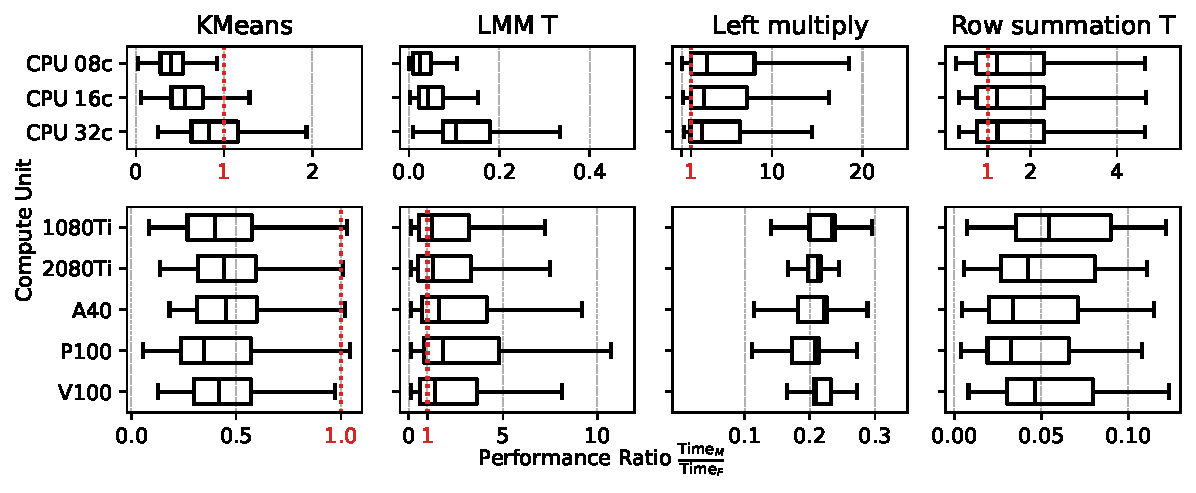
\includegraphics[width=\linewidth]{chapters/05_cost_estimation/figures/motivation_speedup_per_operator_per_gpu.pdf}
    \caption[Performance ratio plotted against hardware]{Performance ratio, of various operators on synthetic data, against hardware. The performance ratio is shown to be affected by hardware choice.}
    \label{fig:5-gpu-characteristics}
\end{figure}
The hardware used for computation impacts the runtime of a program, but here we show it also impacts the F/M trade-off. Different compute unites (i.e., CPU or GPU type) have a different decision boundary for when to use factorization over materialization. This is shown in \autoref{fig:5-gpu-characteristics}. Differing hardware impacts the performance ratio differently per operator. For example, the (mean$\pm$std.) performance ratio of transposed Left Matrix Multiplication on the P100 is $3.03\pm2.70$, while on the V100 it is slightly lower with $2.32\pm2.21$. But, for Left (scalar) multiplication the V100 has the higher performance ratio of $0.21\pm0.04$, against the P100's lower $0.19\pm0.05$.

\begin{table}[ht]
    \centering
    % LTeX: enabled=false
\begin{tabular}{lrrrr}
\toprule
Compute Unit & Mean & Std. Dev. & Count & \% with Speedup \\
\midrule\midrule
CPU 08c & 1.27 & 0.25 & 172 & 1.78\% \\
CPU 16c & 1.32 & 0.34 & 579 & 5.99\% \\
CPU 32c & 1.48 & 0.46 & 2873 & 29.74\% \\
1080Ti & 2.27 & 1.60 & 432 & 4.47\% \\
2080Ti & 1.87 & 1.09 & 425 & 4.40\% \\
A40 & 2.00 & 1.20 & 392 & 4.06\% \\
P100 & 2.52 & 1.84 & 461 & 4.77\% \\
V100 & 1.95 & 1.13 & 404 & 4.18\% \\
\bottomrule
\end{tabular}

    \caption[Performance ratio of ML models for cases where factorization has positive impact.]{Mean performance ratio of ML models for cases where factorization is preferred over Materialization (speedup > 1). This shows hardware choice is a large factor in when to choose factorization over Materialization.}
    \label{tab:5-speedup-per-gpu}
\end{table}

For cases where factorization is preferred over materialization ($\text{Time}_F < \text{Time}_M$), there are large differences between the GPUs. Both the mean performance ratio, and the count of cases where F is faster than M varies greatly, as shown in \autoref{tab:5-speedup-per-gpu}. This shows that the choice of hardware is a large factor in when to choose factorization over materialization.

Another interesting observation can be seen when comparing the performance ratio against the complexity ratio \cite{schijndel_cost_estimation}, for different hardware settings. As explained in \autoref{sec:3-cost-estimation-for-factorized-ml} the complexity is defined as the number of FLOPs needed to perform an operation. The ratio is defined as the complexity of the factorized case divided by the complexity of the materialized case. Thus, per \cite{schijndel_cost_estimation}, the higher this ratio the more beneficial it is to use factorization. However, our experiments show that while this is the case for a lot of operators on CPU, when performing the computations on GPUs this is not always the case. This is shown in \autoref{fig:5-complexity-ratio-vs-performance-ratio}. The next section explores why this is the case.

\begin{figure}[ht]
    \centering
    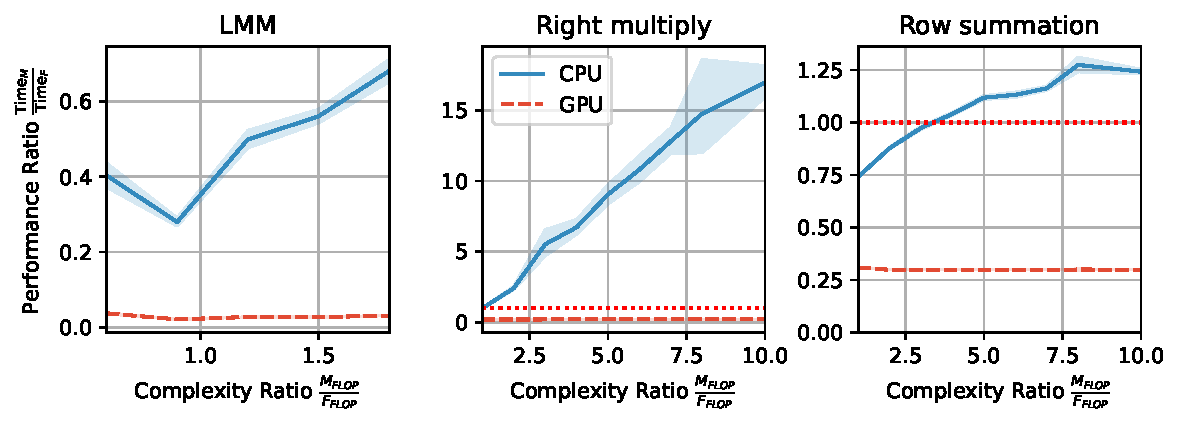
\includegraphics[width=\linewidth]{chapters/05_cost_estimation/figures/motivation_speedup_complexity_ratio.pdf}
    \caption[Performance ratio plotted against complexity ratio]{Performance ratio, of various operators on synthetic data, against complexity ratio, broken down by CPU and GPU. 95\% Confidence interval shown as shaded area. Where a lot of operators show clear correlation between the complexity ratio and the performance ratio on CPU, this is not the case for GPU.}
    \label{fig:5-complexity-ratio-vs-performance-ratio}
\end{figure}


\section{GPU Performance Analysis}
\label{sec:5-gpu-performance-analysis}
A preliminary step for creating an accurate cost model is to understand the performance characteristics of the hardware. This section analyses the profiling metrics collected during the experiments, to understand how the choice of hardware impacts the trade-off between factorization and materialization. A first simple analysis is to compare the memory cost and math cost of the profiled scenarios. Per NVIDIA, a fitting way to estimate the runtime of a GPU program is to compute $max(T_{mem}, T_{math})$. In this formula $T_{mem}$ is the time it takes to transfer data to and from GPU memory, and $T_{math}$ is the time it takes to perform the actual computations. This is in line with the fact that the memory throughput of a GPU is much higher than that of a CPU, and thus the computations are often memory-bound. In this section we show whether this is the case for our experiments, and how we can use this to estimate the runtime of an ML training scenario.

\begin{figure}[ht]
    \centering
    \begin{minipage}{0.50\textwidth}
        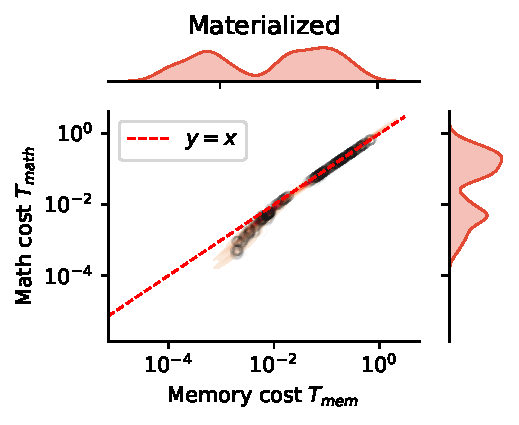
\includegraphics[width=\linewidth]{chapters/05_cost_estimation/figures/profiling-mem-vs-compute-materialized.pdf}
    \end{minipage}\hfill
    \begin{minipage}{0.50\textwidth}
        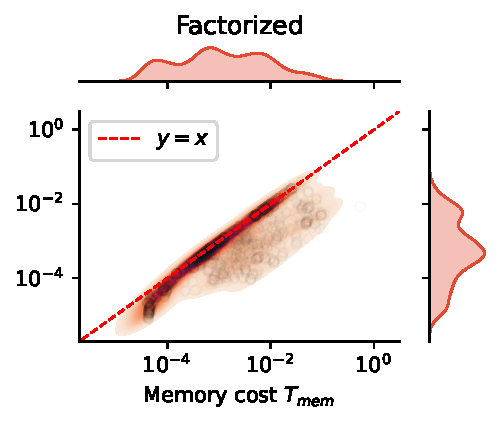
\includegraphics[width=\linewidth]{chapters/05_cost_estimation/figures/profiling-mem-vs-compute-factorized.pdf}
    \end{minipage}
    \caption[Memory cost vs math cost of profiled scenarios]{Memory cost ($T_{mem}$) vs compute cost ($T_{math}$) of profiled scenarios. The memory cost is computed as the total number of bytes read and written to memory divided by the measured average memory bandwidth. The math cost is the number of cycles the Streaming Multiprocessors were active divided by the measured average SM frequency.}
    \label{fig:5-profiling-mem-vs-compute}
\end{figure}

\autoref{fig:5-profiling-mem-vs-compute} shows the distribution of $T_{mem}$ vs $T_{math}$. As expected, these values are highly correlated ($\rho = 0.99$). Almost none of the profiled scenarios have a higher math cost than memory cost, all points are below the $y=x$ line. This shows that the computations are memory-bound, and that the memory cost is a good estimator for the runtime of a scenario. However, the difference between factorization and materialization is substantial. This first becomes obvious when calculating the correlation, for the materialized cases $\rho \text{is} 0.99$, for the factorized cases this is only $0.40$. The cause for this is that with the materialized case the GPU only has to handle a single matrix (or two matrices in the case of matrix multiplication). The normalized matrix used for the factorized case consists of more separate matrices ($S,I,M$), each used in different computations. On average, this reduces both the memory and compute cost. However, it also causes a shift away from the $T_{mem} = T_{math}$ line, as the computations on the different matrices are executed in sequence on the GPU.

\begin{figure}
    \centering
    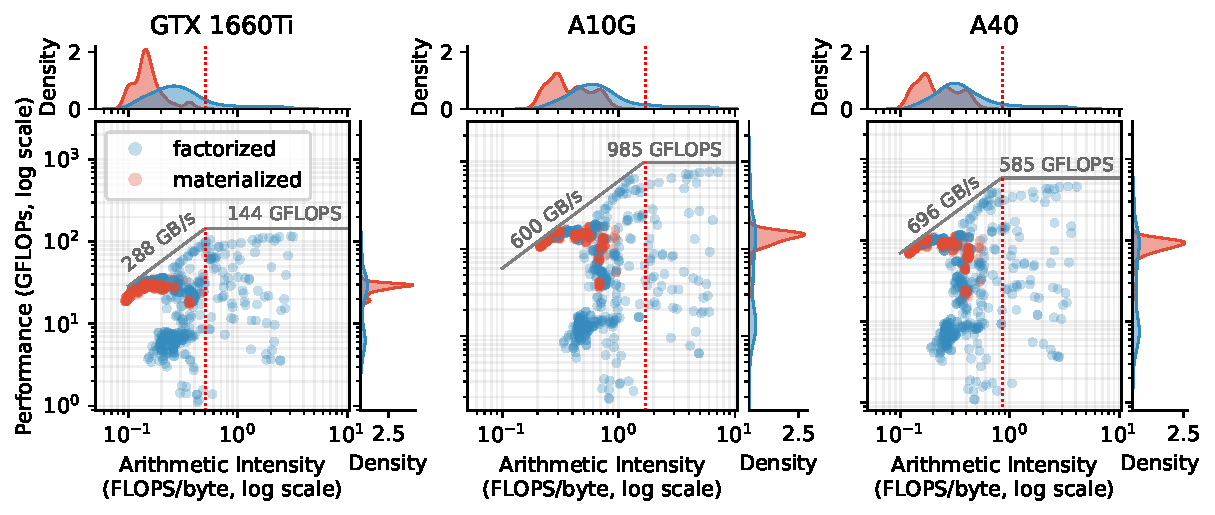
\includegraphics[width=\linewidth]{chapters/05_cost_estimation/figures/roofline-plot.pdf}
    \caption[Roofline chart comparing F/M, per GPU]{Roofline chart showing where the performance of the GPUs lies in the memory-bound vs compute-bound spectrum. The subplots on top and right side of each figure show the distribution along the performance (GFLOPs) and operational intensity (FLOPs/byte) axes. Similar GPU types have similar distributions.}
    \label{fig:5-roofline-plot}
\end{figure}

\subsubsection*{Roofline Model}
Not only the split in metrics between F and M is interesting, but the difference in efficiency between different GPUs is also substantial. A roofline model can be used to create a visualization for this. It is a “model that offers insight insights \ldots on improving parallel software and hardware for floating point computations” \cite{roofline}. The roofline model shows whether an operator on a given scenario is memory- or compute-bound. The x-axis shows arithmetic intensity of a program in FLOPs per byte (in our case a program is an operator executed on a given dataset), the y-axis the (attainable) performance in GFLOPs. The roofline (top line in grey) shows the bound on performance of a given GPU. It is constructed by taking the maximum memory bandwidth and the maximum number of FLOPs the GPU can perform per second. The point where they meet (\textit{ridge point}) tells you the minimum arithmetic intensity needed to fully utilize a GPUs compute capacities. By plotting programs on such a roofline chart one can reason about whether it is compute- or memory-bound by whether it is to the left (memory bound) or to the right of the \textit{ridge point's} x coordinate (compute bound). This is insightful because it shows where the opportunity for optimization lies by identifying bottlenecks.

The roofline charts for the performed profiling experiments are shown in \autoref{fig:5-roofline-plot}. These charts confirm that almost all scenarios are memory-bound. But, the interesting observation from this plot is the impact of GPU type, and the difference between factorization and materialization. The differences between GPUs are most obvious in the right distribution plots. The A10G and A40 are much more powerful GPUs. On the GTX1660Ti most scenarios reach a low compute performance as they hit the memory bound. The A10G and A40, however, have a much higher memory bandwidth. Thus, the scenarios have reach a higher average performance. The gap these plots show between factorization and materialization gives more valuable insights. The materialized operators have lower arithmetic complexity than their factorized equivalents (shown in top density plots). This means that, on average, the factorized operators are less memory-bound, and thus can utilize a larger part of the GPUs compute capacity. However, the factorized operators show a much larger variance in attained performance (right density plots) due to the fact that the operations on different parts of the normalized matrix are not parallelized. These operators can likely be tweaked, so they can take advantage of the GPUs compute capacity more efficiently.

\begin{figure}[ht]
    \centering
    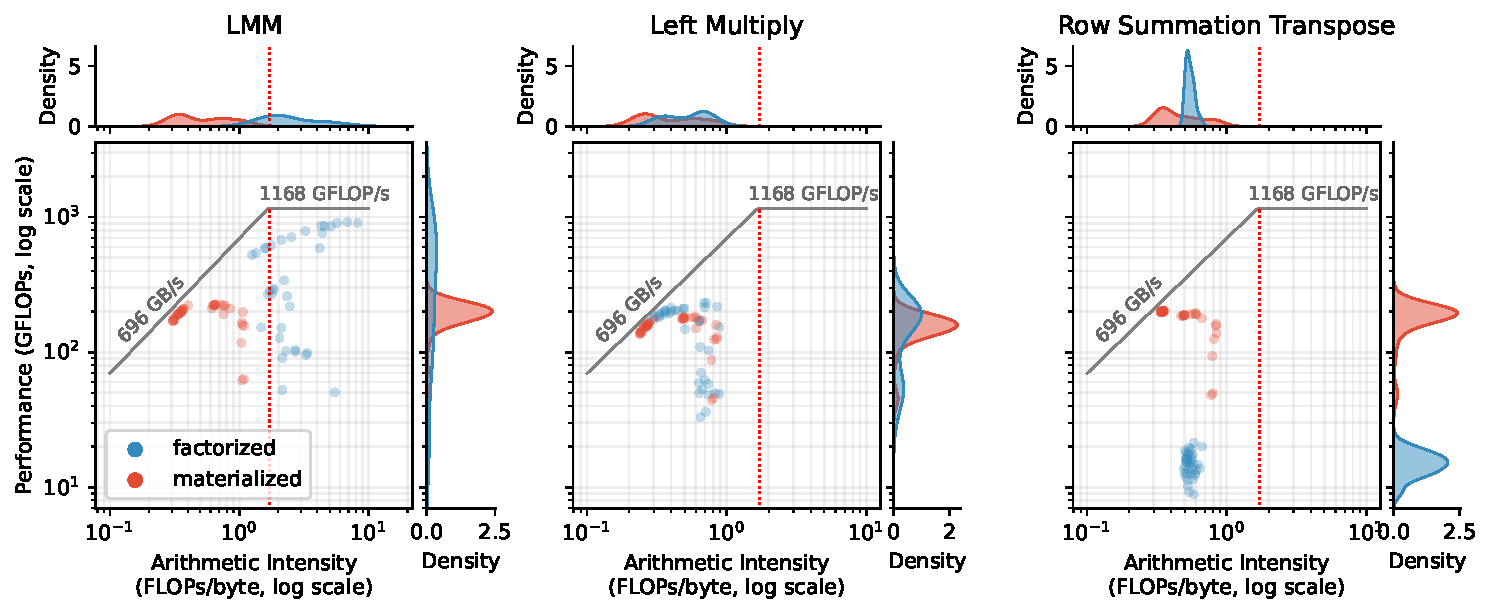
\includegraphics[width=\linewidth]{chapters/05_cost_estimation/figures/roofline-operators.pdf}
    \caption[Roofline chart per operator]{Roofline chart comparing factorization and materialization for Left Matrix Multiplication, Left Scalar Multiplication and Row Summation Transpose. Metrics from NVIDIA A40.}
    \label{fig:5-roofline-operators}
\end{figure}

A roofline chart for a selection of operators is shown in \autoref{fig:5-roofline-operators}. This breakdown per operator further shows the differences between factorization and materialization. Compared to the materialized case, the factorized case of Left Matrix Multiplication shows extremely large variance in performance, which is in line with the use of the normalized matrix explained previously. Although, overall, using factorization seems beneficial for LMM when looking at these profiling metrics (values move to the top and right, indicating higher saturation of the available resources). For Left Scalar Multiplication the gap between F and M is much smaller, which is logical as the factorized case only multiplies the Source matrices with the scalar, which is a simpler operation than the one needed for LMM. The right-most plot shows this limitation even more clearly, showing significantly less utilization of the GPU performance than the materialized case for Transpose Row Summation.

\section{Feature Engineering}
\label{sec:5-feature-engineering}
\todo{
    Data Preprocessing steps
    \begin{enumerate}
        \item Collection of data characteristics
        \item Complexity
        \item ratios: complexity, sparsity
        \item Memory costs from profiling metrics
        \item Computation costs from profiling metrics
    \end{enumerate}
    Finally show schema of the final dataset used for training the models.
}
From our experiments (further detailed in \autoref{sec:6experiment-setup}) we have a dataset with for each scenario (consisting of a dataset, operator, model type F/M,  hardware configuration and the runtime of this scenario). This section details the process of preprocessing and enriching this dataset with additional features. The goal is to create a dataset that can be used to train the cost models. The features we add are based on the profiling metrics collected during the experiments, and the data and model characteristics. The process is visualized in \autoref{fig:5-feature-enrichment}. The feature set is described in \autoref{tab:5-features}.


\subsection{Preprocessing Profiling Metrics}
\begin{figure}[ht]
    \centering
    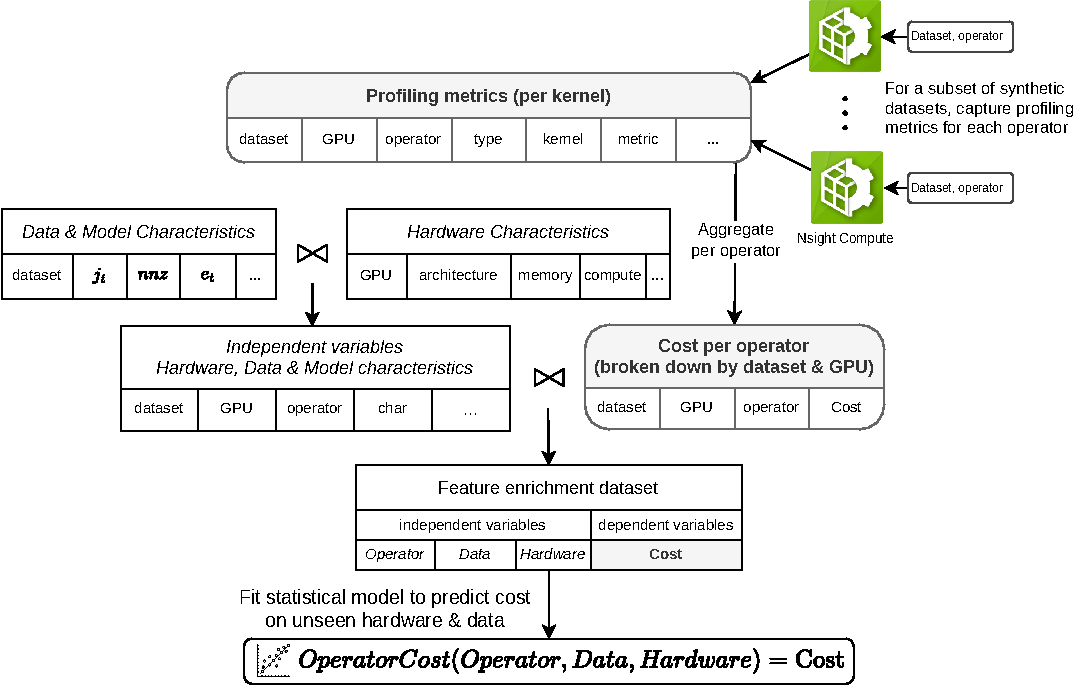
\includegraphics[width=\linewidth]{chapters/05_cost_estimation/figures/feature-engineering.pdf}
    \caption[Feature enrichment workflow]{Workflow of enriching the collected data with additional features from the profiling experiments. Items related to these profiling experiments are \textbf{bolded}, while the features from the data, model \& hardware characteristics are \textit{italicized}.}
    \label{fig:5-feature-enrichment}
\end{figure}

There are two issues with the profiling metrics we have collected. First, the metrics are collected on a per-kernel basis, while we are interested in the performance of a scenario (operator). Second, the metrics are collected for a subset of the scenarios, while we want to have metrics for all scenarios. The process of solving these issues is shown in \autoref{fig:5-feature-enrichment} and detailed here.

This paragraph describes the process of aggregating the kernel-level metrics to operator level metrics, annotated by the “1” in \autoref{fig:5-feature-enrichment}. For each scenario, we sum the metrics that are totals, i.e., the metrics with units nanosecond, byte, or cycle (refer to \autoref{tab:4-profiling-metrics} for which metrics this applies to). The remaining metrics are either a percentage or a measure per second. For these metrics we calculate the weighted average, where the weight is the duration of the kernel. This is done to ensure that the metrics are representative of the total runtime of the scenario.

The second issue is that the metrics are not collected for all scenarios. This is solved by fitting a statistical model to the collected metrics, and using this model to predict the missing metrics. The model is a linear regression model, with the collected, aggregated, metrics as features.

\subsection{Derived Features}
Here we describe the process of generating new features from combinations of independent variables. By combining the multiple collected metrics we can create new features that can be used to train the cost models. The derived features are:

\begin{table}[ht]
    \centering
    \begin{tabular}{p{0.19\linewidth}p{0.37\linewidth}p{0.35\linewidth}}
        \toprule
        Feature                                   & Formula                                                                                                 & Description                                                                                                                                       \\
        \midrule\midrule
        \texttt{dram\_bytes\_sum}                 & $\texttt{dram\_bytes\_read\_sum} + \texttt{dram\_bytes\_write\_sum}$                                    & Total number of bytes read and written to DRAM.                                                                                                   \\
        $T_{mem}$                                 & $\frac{\texttt{dram\_bytes\_sum}}{\texttt{memory\_throughput\_byte\_weighted\_mean}}$                   & Total memory bytes divided by the achieved memory throughput. Gives the cost of the involved memory operators in seconds.                         \\
        $T_{math}$                                & $\frac{\texttt{sm\_active\_cycles\_sum}}{\texttt{sm\_frequency\_weighted\_mean}}$                       & Total active cycles divided by the achieved frequency of the Streaming Multiprocessors. Gives the cost of the involved math operators in seconds. \\
        \texttt{FLOPs}                            & $\frac{\texttt{compute\_throughput\_weighted\_mean}}{100} \times \text{\small{gpu\_processing\_power}}$ & Total number of FLOPs executed in the scenario. Processing power is for double precision.                                                         \\
        \texttt{arithmetic\_-} \texttt{intensity} & $\frac{\texttt{FLOPs} \times \texttt{duration}}{\texttt{dram\_bytes\_sum}}$                             & The number of FLOPs executed per byte read or written to memory.                                                                                  \\

        \bottomrule
    \end{tabular}
    \caption[Derived features]{Overview of computed features. values in \texttt{monospace} are collected through profiling experiments. Features starting with "gpu" are constants for the specific GPU used.}
    \label{tab:5-derived-features}
\end{table}




\begin{table}[ht]
    \centering
    % LTeX: enabled=false
\begin{tabular}{lp{0.23\linewidth}p{0.10\linewidth}>{\footnotesize}p{0.15\linewidth}p{0.08\linewidth}l}
    \toprule
    Dimension                    & Feature                                 & Symbol       & Formula                             & Type & Notes                  \\
    \midrule\midrule
    \multirow[t]{12}{*}{Data}    & Complexity                              & $O_M$, $O_F$ &                                     & N    &                        \\
                                 & Complexity ratio                        &              & $\frac{M_{FLOP}}{F_{FLOP}}$         & N    &                        \\
                                 & Dataset size (rows, columns)            & $r_T, c_T$   &                                     & N    &                        \\
                                 & Feature ratio                           & $\rho$       & $\frac{n_S}{\sum_{k=1}^p n_k} $     & N    &                        \\
                                 & Join type                               & $j_t$        &                                     & C    &                        \\
                                 & Selectivity                             & $\sigma$     & $\frac{\sum_{k=1}^{n}r_{S_k}}{r_T}$ & N    &                        \\
                                 & Sparsity                                & $e_T$        & $\frac{nnz(T)}{r_T\times c_T}$      & N    &                        \\
                                 & Sparsity ratio                          &              & $\frac{e_T}{e_S}$                   & N    &                        \\
                                 & Tuple ratio                             & $\tau$       & $\frac{\sum_{k=1}^p d_k}{d_S}$      & N    &                        \\
                                 & \# Base tables                          & $n$          &                                     & N    &                        \\
                                 & \# Non-zero values                      & $nnz(T)$     & $nnz(S) = \sum_{k=1}^{n}nnz(S_k)$   & N    &                        \\
                                 & \# Sparse base tables ($e < 0.05$)      & $q$          & $|\{S_k \in S| e_{S_k} < 0.05\}|$   & N    & From \cite{MorpheusFI} \\

    \multirow[t]{9}{*}{Hardware} & Arithmetic intensity                    &              &                                     & N    &                        \\
                                 & Compute type                            &              &                                     & C    & CPU, GPU               \\
                                 & FLOPs                                   &              &                                     & N    &                        \\
                                 & GPU memory bandwidth                    &              &                                     & N    &                        \\
                                 & GPU processing power (double precision) &              &                                     & N    &                        \\
                                 & Math cost                               & $T_{math}$   &                                     & N    &                        \\
                                 & Memory cost                             & $T_{mem}$    &                                     & N    &                        \\
                                 & Total bytes                             &              &                                     & N    &                        \\
                                 & \# Cores                                &              &                                     & N    &                        \\

    \multirow[t]{4}{*}{Model}    & Operator                                &              &                                     & C    &                        \\
                                 & Rank                                    & $r$          &                                     & N    & GNMF                   \\
                                 & \# Clusters                             & $k$          &                                     & N    & K-Meanss               \\
                                 & \# Iterations                           & $iter$       &                                     & N    &                        \\

    \bottomrule
\end{tabular}

    \caption[Feature table]{Table showing base, and derived/engineered features used for training the cost models. N stands for numerical, C for categorical.}
    \label{tab:5-features}
\end{table}


\section{Cost Models}
\label{sec:5-cost-models}
\todo{Detail the full process going from data to Cost model, what features where used, and what is the inner architecture?\\Show each of the factors is significant. Data, Hardware, Model parameters.\\Show R2 score to compare between models.}



\subsection{Analytical}
\begin{figure}[ht]
    \centering
    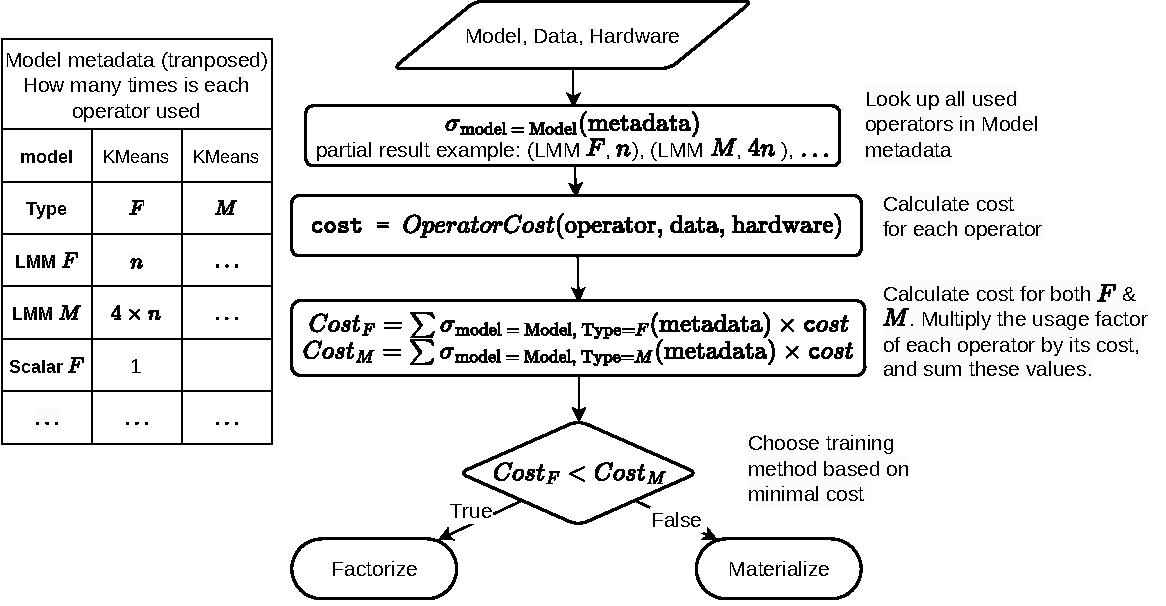
\includegraphics[width=\linewidth]{chapters/05_cost_estimation/figures/analytical-architecture.pdf}
    \caption[Analytical Estimator Architecture]{Architecture of the Analytical Estimator. Shows the control flow of inputs to a final decision on whether to use factorization or materialization. $OperatorCost$ is the function as defined in \autoref{fig:5-feature-enrichment}.}
    \label{fig:5-analytical-architecture}
\end{figure}

Architecture: \autoref{fig:5-analytical-architecture}.

\subsection{Statistical}
The goal for this statistical estimator is to still be explainable, while providing higher performance than the hand tuned decision rules from related works. We use a variety of models, which all use Linear Regression at their core. We start with a singular regressor, and, by drilling down into categorical variables, end up at more complex models, with ensembles of linear regression models.

The architecture of each of the statistical models is shown in \autoref{fig:5-statistical-architecture}. In short, before training the dataset is split by a number of categorical variables (operator type, hardware type or $F$/$M$), or by filtering a part of the dataset. Each final model is a set of Linear Regression models each fit to one of the data subsets. For example, for STAT.3 we train two regressors. One on the factorization scenarios, and one on the materialization scenarios. During inference, each of the regressors is used to predict the runtime of the scenario under test. The output is the predicted materialized time minus the predicted factorized time. This is done to predict the time saved by choosing factorization over materialization. When a categorical variable is not used to split the dataset, it is used as a feature in the model.

\begin{figure}[ht]
    \centering
    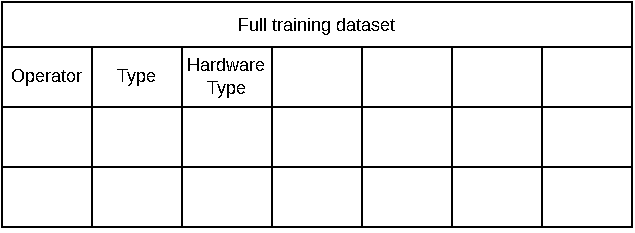
\includegraphics[width=\linewidth]{chapters/05_cost_estimation/figures/statistical-architecture.pdf}
    \caption[Statistical Estimator Architecture]{Architecture of the Statistical Estimators. Shows how the data, and estimators, are split for each model. The final split-level belonging to each respective model is coloured in the same colour. For STAT.5 we show the linear regression ensemble fit to the data. For clarity, we leave this out for the other models. Each box represents a regression model, the same-coloured boxes, connected via dotted lines, are combined into an ensemble to end up with the statistical cost estimators.}
    \label{fig:5-statistical-architecture}
\end{figure}

\subsubsection*{STAT.1 Linear Regressor Fit to Full Training Set}
The first linear regressor is trained on the full training set, which includes all operators. The rationale behind this approach is that there is likely a relationship between the performance of individual operators and the performance of the models in which they are used. By training the regressor on the full set of operators, we aim to capture these relationships and use them to improve the accuracy. This model predicts the time saved by choosing factorization over materialization.

\subsubsection*{STAT.2 Linear Regressor Fit to Model Runtimes}
The second linear regressor is trained on the runtimes of the models. With this model we find whether including the operators adds utility. Like STAT.1, this model predicts the time saved by choosing factorization over materialization.

\subsubsection*{STAT.3 Separate Regressors for F and M}
This model is an ensemble of two linear regressors, one for factorization and one for materialization. By training separate regressors for factorization and materialization, we aim to capture the relationships between independent variables and runtime more explicitly than is done by the previous models. Each internal regressor predicts the runtime of the scenario under test, and the final prediction is which is predicted to be faster.

\subsubsection*{STAT.4 Separate Regressors for each Model Type}
Much like STAT.3 this estimator is also a combination of multiple inner regressors. However, instead of having one regressor for each factorization and materialization, we have one regressor for each model type. This is done to capture the differences in the relationships between independent variables and runtime for different model types. Like the first two models, this model predicts the time saved by choosing factorization over materialization (by predicting whether time is saved by choosing F).

\subsubsection*{STAT.5 Separate Regressors for CPU and GPU}
In previous sections we have shown that the choice of hardware plays a large factor in the trade-off we are researching, therefore it is likely there are differences in the relationships between independent variables and runtime between CPU and GPU. A single linear regression model is likely unable to capture these differences. Therefore, we test the performance of a couple of estimators, one which is only fit to CPU scenario's, and one which is only fit to GPU scenario's.

\subsubsection*{STAT.6 Separate Regressors for F, M and Model Type}
The last version of the statistical model we created is a combination of STAT.4 and STAT.3. By training separate regressors for every combination of factorization, materialization and model type, we allow the models to capture differences between the groups more freely.

\subsubsection*{STAT.7 Separate Regressors For Each Combination of Categories}
The last, most granular, ensemble is one that has a separate regressor for each combination of factorization, materialization, model type and hardware. This is done to capture the differences in the relationships between independent variables and runtime for each combination of the dimensions.


\subsubsection{Statistical Model Evaluation}
\begin{figure}[ht]
    \centering
    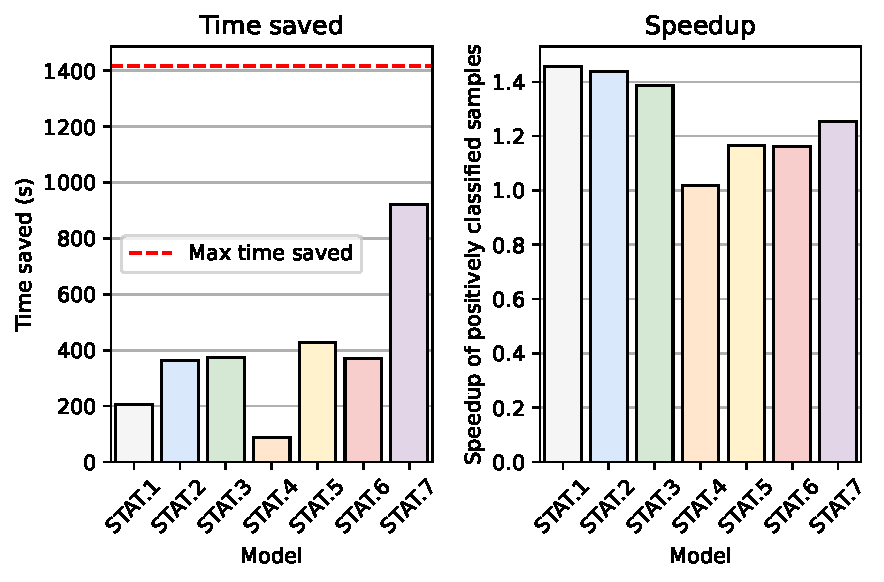
\includegraphics[width=0.75\linewidth]{chapters/05_cost_estimation/figures/stat-models-compare.pdf}
    \caption[Statistical Model Evaluation]{Evaluation of the statistical models on the validation set (synthetic data, only models). The first two plots show statistics of those scenarios where the estimator predicts factorization to be faster. The last plot shows the time saved, as a fraction of the total to-be-saved time (by a perfect estimator), when using this estimator.}
    \label{fig:5-statistical-model-evaluation}
\end{figure}

A performance comparison for the statistical models is shown in \autoref{fig:5-statistical-model-evaluation}. We choose to highlight the cases where the model predicts factorization to be faster, and evaluate the saved time in these cases. Overall, estimators that fit more distinct regressors perform better, showing that each of the chosen categorical variables has impact on the F/M trade-off.

STAT.1-3 show relatively little time saved, but the average speedup of positively classified cases is high. This is due to these models producing either producing a lot of false negatives, missing out on a lot of time saved (STAT.1), or a lot of false positives, which drags down the total time saved (STAT.2,3). STAT.4, split only by model type performs worst of the estimators showing that there is a relation for the speedup between the different model types. Estimators STAT.5,6 both find a relatively large fraction of the positive samples, at the cost of a lot of false positives and negatives. STAT.7, which is the most granular, performs best on the validation set. This is likely due to the fact that it can capture the differences in the relationships between independent variables and runtime for each combination of the dimensions. This estimator is the most complex, but also the most accurate, performing 65\% as well as a perfect cost model would, when looking at the time saved.

\subsection{XGBoost}
The third model type we evaluate is XGBoost \cite{xgboost}, specifically an \texttt{XGBRegressor}\footnote{\url{https://xgboost.readthedocs.io/en/stable/python/python_api.html\#xgboost.XGBRegressor}}. This model is a gradient boosting algorithm, which is an ensemble learning method, using a series of decision trees. We use XGBoost as it has shown excellent performance in a multitude of ML scenarios, as well as showcasing excellent ability for handling unbalanced datasets \cite{xgboost_imbalanced_data}. The model is trained on the same dataset as the statistical models, and uses the same features.

\begin{table}[ht]
    \centering
    \begin{tabular}{llll}
        \toprule
        Model & Target     & Pruning       & Decision Boundary            \\
        \midrule \midrule
        XGB.1 & Runtime    & All operators & $Time_M > Time_F$            \\
        XGB.2 & Runtime    & Only models   &                              \\
        XGB.3 & Speedup    & All operators & $\texttt{speedup} > 1.0$     \\
        XGB.4 & Speedup    & Only model    &                              \\
        XGB.5 & Time saved & All operators & $\texttt{time\_saved} > 0.0$ \\
        XGB.6 & Time saved & Only models   &                              \\
        \bottomrule
    \end{tabular}
    \caption[XGBoost configurations]{Overview of the different configurations for the XGBoost models.}
    \label{tab:5-xgboost-configurations}
\end{table}

We explore a number of different configurations for this model. We explore along two axes: the target variable, and whether to include all operators, or just the model operators in the training dataset. The target variable can be the runtime of the scenario (one target for factorized, one for materialized), the speedup of a scenario, or the time saved by choosing factorization over materialization. The dataset can be pruned only keeping training samples where the operator is one of the model types (KMeans, Logistic Regression, Linear Regression, or GNMF), or keeping all samples. By evaluating multiple models with different configurations, we aim to find the model that best captures the relationships between independent variables and the F/M trade-off. The overview of which model uses which configuration, and how the decision to materialize or factorize is made based on the predicted value(s), is shown in \autoref{tab:5-xgboost-configurations}.

\begin{figure}[ht]
    \centering
    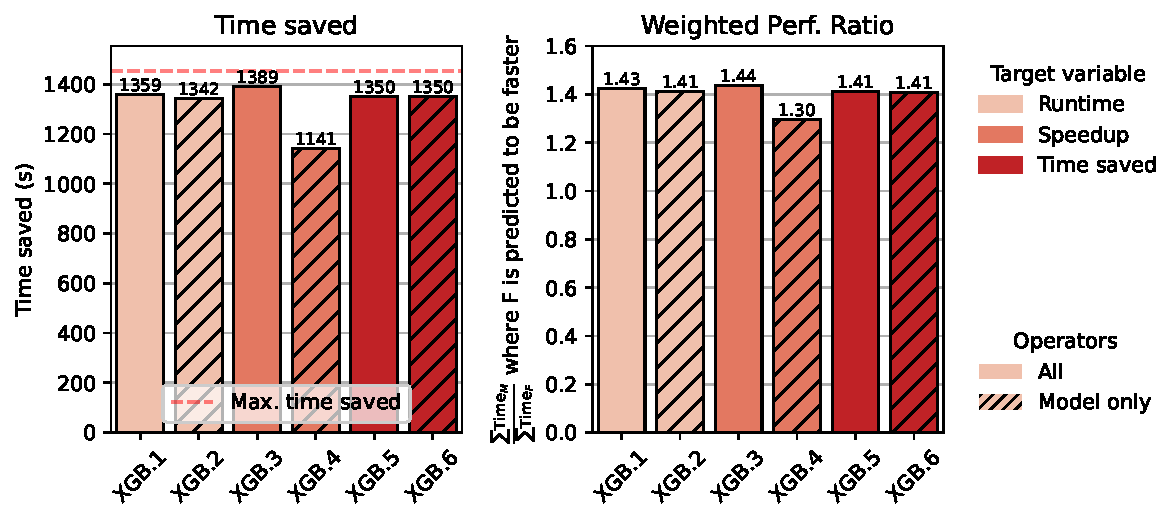
\includegraphics[width=\linewidth]{chapters/05_cost_estimation/figures/xgb-models-compare.pdf}
    \caption[XGBoost Estimator Comparison]{Evaluation of the XGBoost models on the validation set.}
    \label{fig:5-xgboost-evaluation}
\end{figure}

A comparison and evaluation of the XGB models is shown in \autoref{fig:5-xgboost-evaluation}. As expected, as these models are more complex, they perform better than the statistical models. Amongst the XGB models there is little difference in performance on the validation set. There is no significant difference between which target variable is used, or whether all operators are used in the training set. XGB.3, which predicts the speedup of factorization over materialization, barely outperforms the other models, predicting 98\% of the validation scenarios correctly.

\subsection{Hybrid}

\begin{figure}
    \centering
    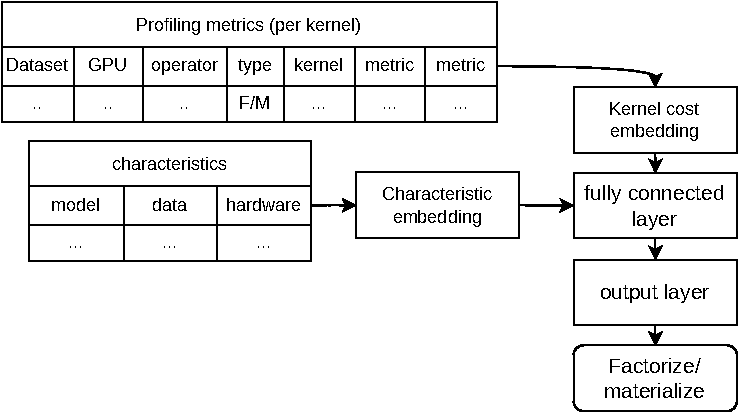
\includegraphics[width=0.7\linewidth]{chapters/05_cost_estimation/figures/hybrid-architecture.pdf}
    \caption[Hybrid Estimator Architecture]{Architecture of the Hybrid Estimator. Inspired by \cite{halide_cost_model}. \todo{Update refine and finalize}.}
    \label{fig:5-hybrid-architecture}
\end{figure}

\subsection{Meta-results}
\todo{Inference speed, training time.}
